\newcommand*{\FactoryPattern}{\begingroup

 %----------------------------------------------------------------------------------------
 %	Factory Method Pattern
 %----------------------------------------------------------------------------------------
\chapter{Factory Method Pattern}
The factory method pattern is categorized as an creational-, object based pattern. One motivation for using the factory method pattern is when external information influence the demand of objects. During the designing process only the time when an object is needed is known, but not what kind of object. Without the factory method pattern the software designer could implement a conditional statement mechanism like shown in list \ref{lst:switchCaseSelection} to cover every possible case.

\lstinputlisting[caption={Switch-case-selection}\label{lst:switchCaseSelection},captionpos=t, backgroundcolor = \color{white}, frame=single, language=C++, firstline=1, lastline=14]{Sourcecode/switch-case-selection.cpp}

\noindent If this selection occurs only once in the whole sourcecode and the number of available objects is small, there is no further demand for refactoring. In projects where the selection occurs on several places, the switch-case-selection can be replaced by a factory call. 

\newpage

\begin{figure}[]{}
\centering
\mbox{\frame{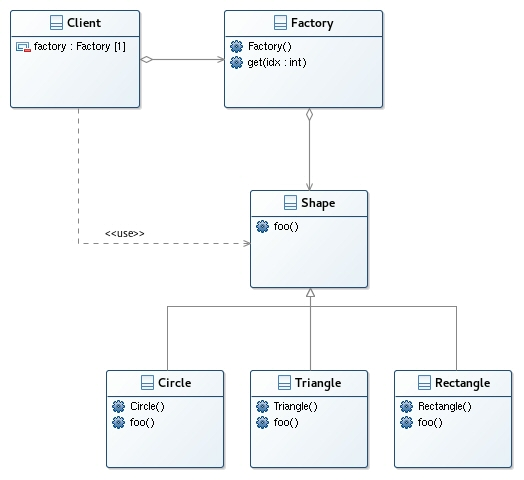
\includegraphics[width=\textwidth]{Images/FactoryPatternSimple.jpg}}}
\caption{Factory method pattern UML}
\label{fig:factoryPatternSimple}
\end{figure}

\noindent Instead of a direct instantiation, the client delegates the request of an object to the factory. The factory instantiates the particular object and returns it to the client. For the concrete classes either an interface or an (abstract) base class is mandatory like shown in figure \ref{fig:factoryPatternSimple}. In this example Shape is the base class of every instantiable sub class. The factory method pattern can be implemented in various different versions. The most straightforward way is probably to move the switch-case-selection, shown in listing \ref{lst:switchCaseSelection}, to the factory.

\newpage

 %----------------------------------------------------------------------------------------
 %	Conditional Statement Implementation
 %----------------------------------------------------------------------------------------
\section{Conditional Statement Implementation}\label{sec:conditionalStatementFactory}

\lstinputlisting[caption={Conditional statement factory C++03}\label{lst:switchCaseSelectionCpp03},captionpos=t, backgroundcolor = \color{white}, frame=single, language=C++, firstline=1, lastline=16]{Sourcecode/conditionalStatementFactory.cpp}

\noindent This version of a factory has several advantages. Firstly, it is easy to read, to implement and to extend. Another advantage is the performance of a switch-case-statement. Many compilers compile the switch-case-statement to a jump table. The result is a performance of T(n) = $\Theta$(1) for finding the requested branch. \cite[cf.][]{Ding2012} For getting a concrete object, the client uses the factory like shown in listing \ref{lst:factoryCallCpp03}.

\lstinputlisting[caption={Factory call C++03}\label{lst:factoryCallCpp03},captionpos=t, backgroundcolor = \color{white}, frame=single, language=C++, firstline=1, lastline=7]{Sourcecode/factoryCallCpp03.cpp}

\noindent The major disadvantage of this implementation is the hard-coded behavior which provides no flexibility and portability. The factory cannot be used with other classes without recompiling. If a projects needs more than one factory for different classes, each of these factories need to be implemented for its own. The implementation in C++11 of the conditional statement factory is very similar except for the replacement of all raw pointers by smart pointers. (Listing \ref{lst:switchCaseSelectionCpp11})

\lstinputlisting[caption={Conditional statement factory C++11}\label{lst:switchCaseSelectionCpp11},captionpos=t, backgroundcolor = \color{white}, frame=single, language=C++, firstline=1, lastline=19]{Sourcecode/conditionalStatementFactoryCpp11.cpp}
\FloatBarrier

 %----------------------------------------------------------------------------------------
 %	Smart Pointer
 %----------------------------------------------------------------------------------------
\subsection{Smart Pointer}\label{sec:smartPointer}
\noindent As mentioned in section \ref{sec:modernCplusplus} guidelines for C++11 recommend the use of smart pointers instead of raw pointers. The main reason for this is the tendency of getting memory leaks with raw pointers. Opportunities for getting memory leaks vary. For example if the software designer allocates memory with new and forgets to call delete before leaving the scope, only the pointer will be deleted. The allocated memory still exists in the heap. Another fatal situation can happen when an exception occurs before calling the delete. The software designer must take care of this situation. \cite[cf.][848 - 849]{Kirch2015} With smart pointers such situations become more safe. Instead of directly allocating memory the user creates a smart pointer which manages the dynamic allocated objects or data types. C++11 provides three significant types of smart pointers. The Unique pointer, shared pointer and weak pointer.

 %----------------------------------------------------------------------------------------
 %	Unique Pointer
 %----------------------------------------------------------------------------------------
\subsubsection{Unique Pointer (unique\_ptr)}\label{sec:uniquePointer}
\begin{center}\textbf{Example:} unique\_ptr<int> myUniquePtr = make\_unique<int>(42);\end{center}
The destructor of a unique pointer deletes the managed object, regardless whether another pointer refers to that object or not. Therefore a unique pointer does not have a copy constructer, so that sharing the membership of the managed object is not possible. The only way to pass the membership is by using the move constructor. With the move constructor the current unique pointer loses the membership and the new unique pointer is the new unique membership holder of the managed object. Unique pointer are useful for managing ressources like text files. \cite[cf.][850 - 853]{Kirch2015} The size of a unique pointer is 8 bytes\footnote{Every memory size declaration within this document bases on a 64bit system.} for the reference to the managed object. 

 %----------------------------------------------------------------------------------------
 %	Shared Pointer
 %----------------------------------------------------------------------------------------
\subsubsection{Shared Pointer (shared\_ptr)}\label{sec:sharedPointer}
\begin{center}\textbf{Example:} shared\_ptr<int> mySharedPtr = make\_shared<int>(42);\end{center}
Unlike unique pointers, share pointers allow to share the membership of the managed object. To guarantee that the managed object will not be destroyed as long as at least one pointer refers to that, and will be destroyed when the last pointer stops refering to the managed object, the shared pointer uses a reference counter. The reference counter increases when a new pointer refers to the managed object and decreases when a pointer stops refering to the managed object. If the reference counter becomes zero, the object will be destroyed. A disadvantage of a shared pointer compared with a raw pointer is an overhead of allocation time because in addition to the memory for the managed object the shared pointer must also allocate memory for the reference counter. The \emph{make\_shared<>()} function reduces this overhead by allocating the memory in one block. \cite[cf.][854 - 861]{Kirch2015} The size of a shared pointer is 16 bytes. 8 bytes for the reference to the managed object and 8 bytes for the reference to the reference counter. In addition to this the shared pointer also allocates 8 bytes for the reference counter.

 %----------------------------------------------------------------------------------------
 %	Weak Pointer
 %----------------------------------------------------------------------------------------
\subsubsection{Weak Pointer (weak\_ptr)}\label{sec:weakPointer}
\begin{center}\textbf{Example:} weak\_ptr<int> myWeakPtr = mySharedPtr;\end{center}
A weak pointer can only manage objects which are already managed by at least one shared pointer. It has no effect on the reference counter. This means if the last shared pointer stops refering to the managed object, the object will be destroyed and the weak pointer refers to unallocated memory. Weak pointers are useful when several objects have a direct or indirect reference to each other. In this case the reference counter cannot reach zero. Using weak pointer instead, removes the dependency of these objects. \cite[cf.][862 - 863]{Kirch2015} The size of the weak pointer is 16 bytes. As already mentioned the weak pointer has no effect on the reference counter, but it provides the option for a cast to a shared pointer. In this case it is necessary to know about the reference counter. Therefore the weak pointer contains an reference to the reference counter.

 %----------------------------------------------------------------------------------------
 %	Type Inference with auto
 %----------------------------------------------------------------------------------------
\subsection{Type Inference with auto}\label{sec:typeDeduction}
With C++11 not only the factory has changed. A look at the use of the factory (listing \ref{lst:factoryCallCpp11}) shows that the explicit type declaration was replaced by the placeholder \emph{auto}. \emph{auto} is part of the generic programming facilities of C++. As long as the compiler can determine the correct data type at compile time, \emph{auto} can be used for type declaration as well as for the declaration as a return-type. \cite[cf.][210 - 211]{Kirch2015} Type inference benefits the maintaining and modifying process of the sourcecode. 

\lstinputlisting[caption={Factory call C++11}\label{lst:factoryCallCpp11},captionpos=t, backgroundcolor = \color{white}, frame=single, language=C++, firstline=1, lastline=7]{Sourcecode/factoryCallCpp11.cpp}

\FloatBarrier

%----------------------------------------------------------------------------------------
%	Timing for conditional statement implementation
%----------------------------------------------------------------------------------------
\subsection{Timing}\label{sec:timingConditionalStatementFactory}

\begin{figure}[h]{}
\centering
\mbox{\frame{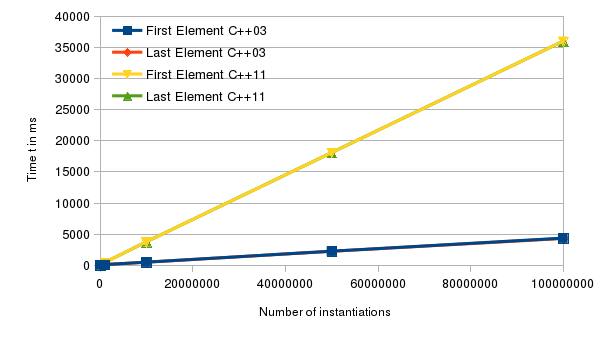
\includegraphics[width=\textwidth]{Images/ConditionalStatementFactoryTiming.png}}}
\caption{Conditional statement factory timing}
\label{fig:conditionalStatementFactoryTiming}
\end{figure}

\noindent Figure \ref{fig:conditionalStatementFactoryTiming} compares the implementation of listing \ref{lst:switchCaseSelectionCpp03} with listing \ref{lst:switchCaseSelectionCpp11}. Each factory manages 100 classes. For the instantiation of 10,000 objects the C++03 version needs about 0.72ms and the C++11 version needs about 5.1ms. For the instantiation of 100,000,000 objects the C++03 version needs about 4.3 seconds and the C++11 version needs about 35.9 seconds. %So using smart pointers brings a disadvantage in timing with a factor of about 7 to 8.
The complexity of both versions is constant. T(N) = $\Theta$(1).
 
\begin{table}[h]\begin{center}
\begin{tabular}{|c|c|c|}\hline
\textbf{Category} & \textbf{Percentage} & \textbf{Time in s}\\
\hline
Factory & 19.18 & 0.81\\
\hline
Shape & 61.18 & 2.60\\
\hline
Main & 17.27 & 0.73\\
\hline
Other & 2.37 & 0.10\\
\hline
\end{tabular}
\caption{Conditional statement factory timing distribution C++03}
\label{tab:ConditionalStatementFactoryTimingDistributionCpp03}
\end{center}\end{table}

\begin{table}[h]\begin{center}
\begin{tabular}{|c|c|c|}\hline
\textbf{Category} & \textbf{Percentage} & \textbf{Time in s}\\
\hline
Factoy & 1.33 & 0.47\\
\hline
Smart pointer & 82.28 & 29.53\\
\hline
Shape & 2.87 & 1.03\\
\hline
Main & 2.82 & 1.01\\
\hline
Other & 10.7 & 3.84\\
\hline
\end{tabular}
\caption{Conditional statement factory timing distribution C++11}
\label{tab:ConditionalStatementFactoryTimingDistributionCpp11}
\end{center}\end{table}

\FloatBarrier 

\noindent The timing analysis, made with the C++ profiler gprof, gives an idea of the root of this overhead of execution time. As shown in table \ref{tab:ConditionalStatementFactoryTimingDistributionCpp03} with about 61\% and 2.6 seconds for 100,000,000 objects Shape causes the biggest part of the C++03 implementation. Within the C++11 implementation table \ref{tab:ConditionalStatementFactoryTimingDistributionCpp11} shows that the use of smart pointers has a big effect on the execution time. With about 82\% and 29.5 secondes for 100,000,000 objects the execution time for using smart pointers is about 10 times as much as the time for Factory, Shape and main together. The amount of operations within the C++11 implementation, which is not explicitly categorisable, takes about 10\% and 3.8 seconds of the total execution time. 

%The profiling output of Eclipse (Figure \ref{fig:conditionalStatementFactoryProfilingCpp03} and \ref{fig:conditionalStatementFactoryProfilingCpp11}), analyzed with the profiler gprof, gives an idea of the root of this overhead of execution time. As shown in table \ref{tab:ConditionalStatementFactoryTimingDistributionCpp03} with 61\% and 2.6 seconds for 100,000,000 objects Shape causes the biggest part of the C++03 implementation. Within the C++11 implementation table \ref{tab:ConditionalStatementFactoryTimingDistributionCpp11} shows that the use of smart pointers has a big effect on the execution time. With 82\% and 29.5 secondes for 100,000,000 objects the execution time for using smart pointers is about 10 times as much as the time for Factory, Shape and main together.

%The profiling output of the C++11 implemententation (Figure \ref{fig:conditionalStatementFactoryProfilingCpp11}) compared with the profiling output of the C++03 implementation (Figure \ref{fig:conditionalStatementFactoryProfilingCpp03}) shows that the overhead of execution time with a factor of about 7 to 8, mainly comes from the usage of smart pointers including the allocation of memory. The explicit execution time of the factory becomes a marginal part of about 1\% of the total execution time. 

%----------------------------------------------------------------------------------------
%	Memory Consumption for conditional statement implementation
%----------------------------------------------------------------------------------------
\subsection{Memory Consumption}\label{sec:memoryConsumptionConditionalStatementFactory}
\noindent As shown in figure \ref{fig:conditionalStatementFactoryMemoryConsumption} neither the C++03 implementation nor the C++11 implementation of the factory cause an memory overhead. Depending on what kind of smart pointers will be used within th C++11 implementation the heap memory overhead for every instantiated object will be either 0 byte or 8 bytes.

\FloatBarrier

\begin{figure}[h]{}
\centering
\mbox{\frame{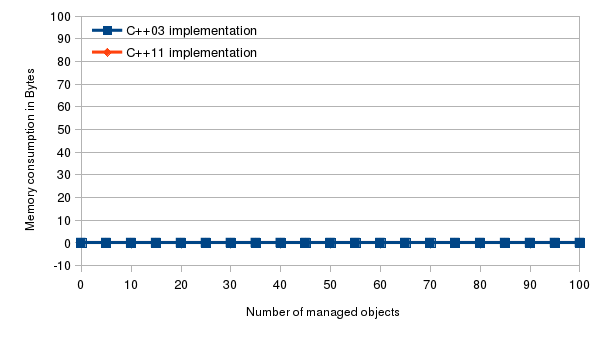
\includegraphics[width=\textwidth]{Images/FactoryPatternSimpleMemoryConsumption.png}}}
\caption{Conditional statement factory memory consumption}
\label{fig:conditionalStatementFactoryMemoryConsumption}
\end{figure}
 
\FloatBarrier

%----------------------------------------------------------------------------------------
%	Clone Factory Implementation
%----------------------------------------------------------------------------------------
\section{Clone Factory Implementation}\label{sec:cloneFactory}
A clone factory manages already instantiated objects. Therefore the factory needs a method for adding objects at runtime. (Shown in figure \ref{fig:factoryPatternClone})

\begin{figure}[h]{}
\centering
\mbox{\frame{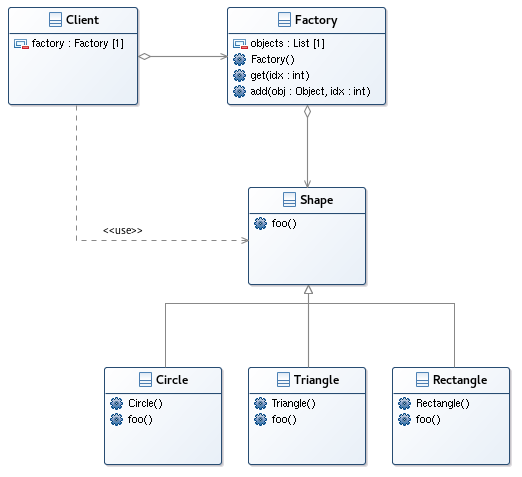
\includegraphics[width=\textwidth]{Images/FactoryPatternClone.png}}}
\caption{Factory method pattern UML including add() method}
\label{fig:factoryPatternClone}
\end{figure}

\noindent If the client requests an object, the factory creates a copy of its managed object and returns the copy. An advantage of this implementation is the flexibility. Objects can be added and removed at runtime. This allows to use the factory more dynamically and to instantiate more than one factories with different managed objects. A basic implementation is shown in listing \ref{lst:cloneFactoryImplementationCpp03}.

\newpage

\lstinputlisting[caption={Clone factory implementation C++03}\label{lst:cloneFactoryImplementationCpp03},captionpos=t, backgroundcolor = \color{white}, frame=single, language=C++, firstline=1, lastline=52]{Sourcecode/cloneFactoryCpp03.cpp}

\noindent This implementation works with a helper class (Cloner) for managing the objects. By adding an object the factory wrappes this object into a Cloner object and stores this within a vector list. The Clone factory requires a consideration of modifying the copy constructor. (Listing \ref{lst:copyConstructorCpp03}) 

\noindent\\ For developing exception-safe code it is neccessary to consider the ownership policy 'Rule of Three'. The Rule of Three says that if either the copy constructor, copy assignment operator or the destructor of a class had to be defined by the software designer, then all of these three parts have to be defined by the software designer. This makes copying objects error-prone because every modification of the object requires an update of the copy constructor, copy assignment operator and destructor. The software designer also has to decide wheter a dynamic allocated data type shall be copied as shallow copy or deep copy. A shallow copy copies the value of the pointer. So both objects, the original object and the copy, will have a pointer to exactly the same memory address. A deep copy allocates new memory and copies the value of the memory, where the pointer refers to, to the new allocated memory. So both objects are pointing to different memory addresses.

\newpage

\lstinputlisting[caption={Rule of Three}\label{lst:copyConstructorCpp03},captionpos=t, backgroundcolor = \color{white}, frame=single, language=C++, firstline=1, lastline=30]{Sourcecode/copyConstructorCpp03.cpp}

\noindent Because of the instantiated objects, the clone factory implementation has a higher memory consumption. The C++11 version of the clone factory (listing \ref{lst:cloneFactoryImplementationCpp11}) implementation contains minor changes. 

\newpage

\lstinputlisting[caption={Clone factory implementation C++11}\label{lst:cloneFactoryImplementationCpp11},captionpos=t, backgroundcolor = \color{white}, frame=single, language=C++, firstline=1, lastline=49]{Sourcecode/cloneFactoryCpp11.cpp}

\noindent As already seen and explained in chapter \ref{sec:conditionalStatementFactory}, all raw pointers were replaced by smart pointers. New is the use of an unordered map instead of a vector list. 

%----------------------------------------------------------------------------------------
%	Unordered Map
%----------------------------------------------------------------------------------------
\subsection{Unordered Map}\label{sec:unorderedMap}
An unordered map is an unordered associative container. This means the unordered map manages the objects within a hash-table. (Figure \ref{fig:hashTable})

\begin{figure}[h]{}
\centering
\mbox{\frame{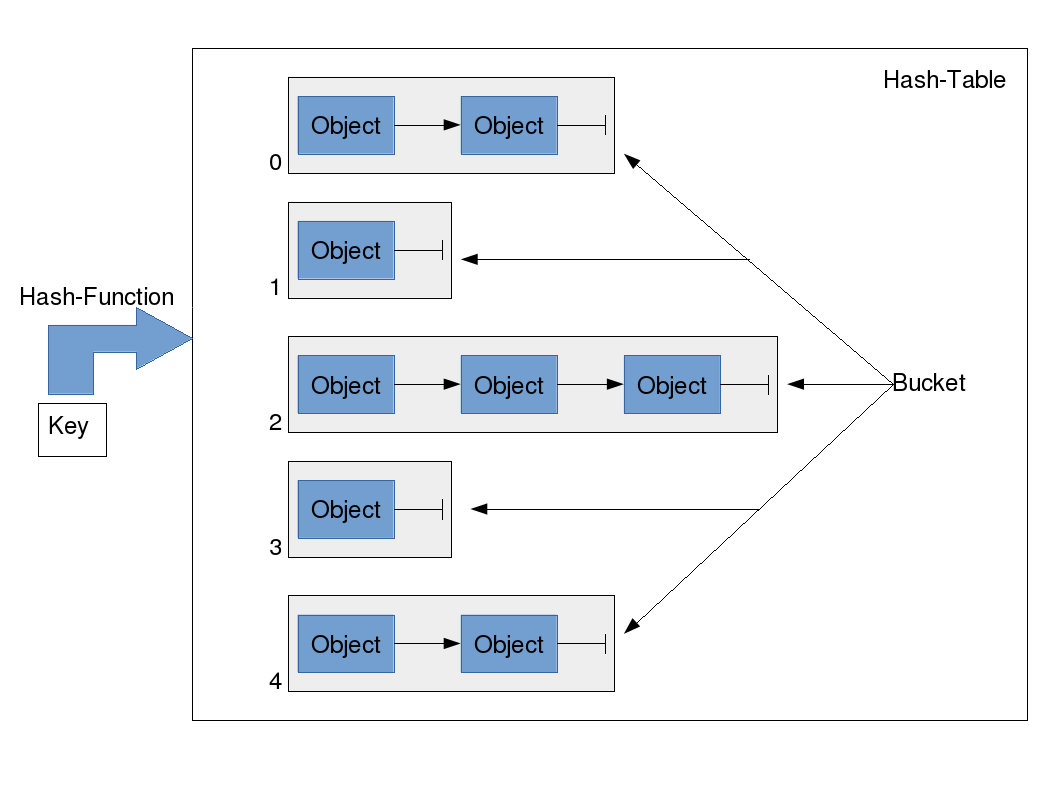
\includegraphics[width=\textwidth]{Images/HashTable.png}}}
\caption{Hash-table \cite[][828]{Kirch2015}}
\label{fig:hashTable}
\end{figure}

\noindent The hash-table consists of entries, named buckets. Each bucket stores the managed objects in a linked list. A hash-function converts the key into a value of type \emph{size\_t}. This value defines in which bucket the object will be stored. With the linked list one bucket can store more than one object at the time. The efficiency of a hash-table depends on the distribution of the objects. In average each bucket contains only one object. In this case the complexity of seek time is T(n) = O(1). In worst case only one bucket contains all object. The seek time is linear so the complexity is T(n) = O(n). At the beginning the hash-table consists of a number b of buckets. If the loadfactor 

\begin{equation}
  loadfactor = n / b
  \label{eq:loadfactor}
\end{equation}

\noindent exceeds a defined threshold with a number n of objects, the hash-table will be reorganized with a new number b of buckets. \cite[cf.][828 - 829]{Kirch2015}

\FloatBarrier

%----------------------------------------------------------------------------------------
%	Rvalue Reference
%----------------------------------------------------------------------------------------
\subsection{Rvalue Reference}\label{sec:rvalueReference}
C++11 provides the option to explicitly define rvalues. Unlike lvalues, rvalues do not have a memory address. 

\lstinputlisting[caption={Lvalue example}\label{lst:lvalueExample},captionpos=t, backgroundcolor = \color{white}, frame=single, language=C++, firstline=1, lastline=2]{Sourcecode/rvalueAndLvalue.cpp}

\lstinputlisting[caption={Rvalue example}\label{lst:rvalueExample},captionpos=t, backgroundcolor = \color{white}, frame=single, language=C++, firstline=4, lastline=4]{Sourcecode/rvalueAndLvalue.cpp} 

\noindent Listing \ref{lst:lvalueExample} shows an example of a typical lvalue. The string does have a name and a memory address. Multiple modifications can be done. Listing \ref{lst:rvalueExample} shows an example of an rvalue. It exists only temporarily and after passing it to the function, the client is not able to do any more with the string because it does not have a name and a memory address. Rvalues are not new. New is the rvalue reference. 

\lstinputlisting[caption={Rvalue reference example}\label{lst:rvalueReferenceExample},captionpos=t, backgroundcolor = \color{white}, frame=single, language=C++, firstline=6, lastline=8]{Sourcecode/rvalueAndLvalue.cpp} 

\noindent The function \emph{foo} (listing \ref{lst:rvalueExample}) only accepts strings as rvalue as parameter. So the call of listing \ref{lst:lvalueExample} would cause a compiler error because \emph{st} is not an rvalue. An rvalue reference makes sure that a reference is not used anymore outside of the function. \cite[cf.][32 - 33]{Pohmann2013} For passing an lvalue as rvalue, C++11 provides the function move to cast an lvalue to an rvalue reference. (Listing \ref{lst:moveExample}) The function forward provides the option to cast an rvalue reference to an rvalue.

\lstinputlisting[caption={Move example}\label{lst:moveExample},captionpos=t, backgroundcolor = \color{white}, frame=single, language=C++, firstline=10, lastline=11]{Sourcecode/rvalueAndLvalue.cpp} 

\noindent as shown in listing \ref{lst:moveExample} by casting an lvalue to an rvalue the string \emph{st} can be passed to the function \emph{foo}. The software designer must consider, the function implies that the parameter is an rvalue and not needed anymore outside of a function. Classes will be extended by a move constructor and a move assignment operator for managing rvalue references. These extend the Rule of Three ownership policy to the Rule of Five. The clone factory always keeps its managed objects. Therefore the visibility of  move constructor and move assignment operator must be set to private. (Listing \ref{lst:moveConstructor})

\newpage

\lstinputlisting[caption={Move constructor and move assignment operator}\label{lst:moveConstructor},captionpos=t, backgroundcolor = \color{white}, frame=single, language=C++, firstline=2, lastline=32]{Sourcecode/moveConstructorCpp11.cpp} 

\newpage

%----------------------------------------------------------------------------------------
%	Timing for Clone Factory implementation
%----------------------------------------------------------------------------------------
\subsection{Timing}\label{sec:timingCloneFactory}

\begin{figure}[h]{}
\centering
\mbox{\frame{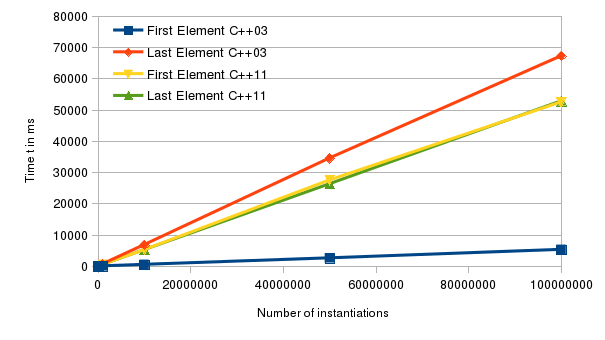
\includegraphics[width=\textwidth]{Images/FactoryPatternCloneTiming.png}}}
\caption{Clone factory timing}
\label{fig:cloneFactoryTiming}
\end{figure}

\noindent Figure \ref{fig:cloneFactoryTiming} compares the implementation of listing \ref{lst:cloneFactoryImplementationCpp03} with listing \ref{lst:cloneFactoryImplementationCpp11}. The seek complexity for finding the requested object within the vector with 100 entries is T(n) = O(n) for the C++03 implementation. Because of the hash-table, the unordered map has a seek complexity of T(n) = O(1). Nevertheless, in average the C++11 implementation is still slower than the C++03 implementation. For cloning 100,000,000 objects, where the requested object always is on the first place within the vector, the C++03 implementation needs about 5.3 second. The farther back the object is in the vector, the longer it takes to find it. So for cloning 100,000,000 objects, where the requested object always is on the last possible place within the vector, the clone factory needs about 67 second. More than 10 times as much as in best case. The C++11 implementation needs constantly 52 seconds for cloning 100,000,000 objects.

\noindent\\ The profiling output (Table \ref{tab:CloneFactoryTimingDistributionCpp03}) shows the distribution of timing of the C++03 in the worst case scenario. With about 96\% and 64.9 seconds the factory causes the biggest part of the execution time. The profiling output (Table \ref{tab:CloneFactoryTimingDistributionCpp11}) of the C++11 implementation shows that the execution time of the factory decreased. The main reason for this is the use of the unordered map. But the use of smart pointers increases the execution time by 38.6 seconds and makes about 73\% of the total execution time. The amount of not explicitly categorisable operations takes about 6\% and 3.24 seconds of the total execution time.

\begin{table}[h]\begin{center}
\begin{tabular}{|c|c|c|}\hline
\textbf{Category} & \textbf{Percentage} & \textbf{Time in s}\\
\hline
Factory & 96.55 & 64.90\\
\hline
Shape & 2.59 & 1.74\\
\hline
Main & 0.86 & 0.57\\
\hline
Other & 0.00 & 0.00\\
\hline
\end{tabular}
\caption{Clone factory timing distribution C++03}
\label{tab:CloneFactoryTimingDistributionCpp03}
\end{center}\end{table}

\begin{table}[h]\begin{center}
\begin{tabular}{|c|c|c|}\hline
\textbf{Category} & \textbf{Percentage} & \textbf{Time in s}\\
\hline
Factory & 18.01 & 9.51\\
\hline
Smart pointer & 73.1 & 38.61\\
\hline
Shape & 1.24 & 0.65\\
\hline
Main & 1.35 & 0.71\\
\hline
Other & 6.14 & 3.24\\
\hline
\end{tabular}
\caption{Clone factory timing distribution C++11}
\label{tab:CloneFactoryTimingDistributionCpp11}
\end{center}\end{table}


 %The profiling output of the C++11 implementation (Figure \ref{fig:cloneFactoryProfilingCpp11}) compared with the profiling output of the C++03 implementation (Listing \ref{fig:cloneFactoryProfilingCpp03}) shows similar results like already seen at the conditional statement implementation of chapter \ref{sec:conditionalStatementFactory}. Most of the overhead of execution time occurs by using smart pointers. Figure \ref{fig:cloneFactoryProfilingCpp11} also shows that the hashtable of the unordered\_map also contributes to the execution time. The row with name '??' contains several uncategorised operations (Figure \ref{fig:cloneFactoryProfilingUncategorisedCpp11}) with a major part of typeinfo and a minor part of the vtables of the objects. 

\FloatBarrier

%----------------------------------------------------------------------------------------
%	Memory Consumption for Clone Factory implementation
%----------------------------------------------------------------------------------------
\subsection{Memory Consumption}\label{sec:memoryConsumptionCloneFactory}
\noindent Unlike the conditional statement implementation, a clone factory manages objects. For each object the factory allocates memory. Figure \ref{fig:cloneFactoryMemoryConsumption} shows the memory overhead of the factory depending on the number of managed objects. In general the C++11 implementation causes a bigger memory overhead than the C++03 implementation. This overhead is caused by the use of an unordered map including a hash-table. As mentioned in section \ref{sec:unorderedMap} the hash-table of the unordered map consists of a number of buckets, depending on the loadfactor (Equation \ref{eq:loadfactor}). When the loadfactor reaches a defined value, the unordered map allocates new memory for having more buckets. This allocation can be observed in figure \ref{fig:cloneFactoryMemoryConsumption} between 20 and 25, 45 and 50 as well as between 95 and 100 managed objects. The \emph{std::vector} also allocates more memory than actually needed to reduce the number of allocations on growing. \cite[cf.][]{CppReference2014_vector}  Figure \ref{fig:cloneFactoryMemoryConsumption} also shows these allocations between 15 and 20, 30 and 35 as well as between 60 and 65 managed objects. The size of the particular objects has also has an impact of the memory consumption of the clone Factory. 

\begin{figure}[h]{}
\centering
\mbox{\frame{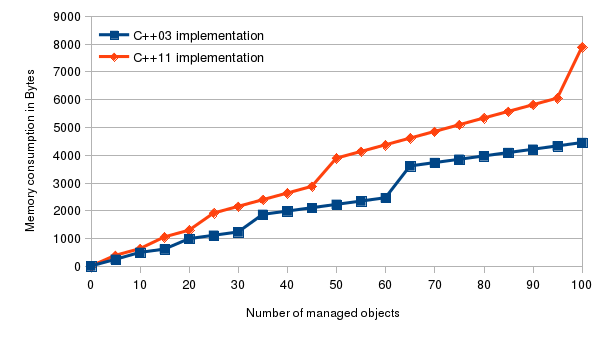
\includegraphics[width=\textwidth]{Images/FactoryPatternCloneMemoryConsumption.png}}}
\caption{Clone factory memory consumption}
\label{fig:cloneFactoryMemoryConsumption}
\end{figure}
 
\FloatBarrier

%----------------------------------------------------------------------------------------
%	Lambda Implementation
%----------------------------------------------------------------------------------------
\section{Lambda Implementation}\label{sec:lambdaFactory}
\noindent As mentioned in section \ref{sec:cloneFactory} cloning objects is error-prone because of the demand for maintenance of destructor, copy constructor and copy assignment operator. In addition, depending on the size and the number of the managed objects the clone factory tends to have a high memory consumption. With establishing lambda expressions, C++11 provides an alternative implementation. (Listing \ref{lst:lambdaImplementation})

\lstinputlisting[caption={Lambda implementation C++11}\label{lst:lambdaImplementation},captionpos=t, backgroundcolor = \color{white}, frame=single, language=C++, firstline=1, lastline=26]{Sourcecode/lambdaFactory11.cpp} 

%----------------------------------------------------------------------------------------
%	Lambda Expression
%----------------------------------------------------------------------------------------
\subsection{Lambda Expression}\label{sec:LambdaExpression}
\noindent A lambda expression is a local anonymous function with access to objects and variables in its environment. \cite[cf.][914 - 915]{Kirch2015}

\lstinputlisting[caption={Lambda expression syntax}\label{lst:lambdaExpression},captionpos=t, backgroundcolor = \color{white}, frame=single, firstline=1, lastline=2]{Sourcecode/LambdaExpression.cpp} 

\noindent The syntax of a lambda expression (Listing \ref{lst:lambdaExpression}) consists of the following parts:


\begin{itemize}
  \item\textbf{[capture]} defines the access to its environment. It can be either [] no access, [=] access by value or [\&] access by reference. Also combinations and access to particular objects are possible. (Example: [=,\&var] defines general access by value except for the variable \emph{var}, which is passed by reference.)
  \item\textbf{(parameterlist)} contains the declaration of the function's parameter. 
  \item\textbf{mutable} is optional and defines whether objects, passed by value, are  declared as const or not. 
  \item\textbf{noexcept} is optional and defines whether the function is able to throw an exception or not.
  \item\textbf{return-type} is optional and explicitly defines the return-type. Without defining it explicitly, the return-type can be determined from the return value.
  \item\textbf{function body} contains the implementation of the function.
\end{itemize}

\noindent The call of a lambda expression can be occur later than the declaration. Because of that, lambda expressions can be stored passed as a parameter. For this C++11 provides a generic wrapper named \emph{function}. \emph{function} is able to take a lambda expression. It gives the lambda expression a memory address. Line 20 and 21 of listing \ref{lst:lambdaImplementation} shows the declaration of a lambda expression which instantiates a smart pointer refering to an object of a generic type T and stores it into a container. If the object of type T is actually needed, the stored lambda expression can be called which instantiates and returns the requested smart pointer. 

%----------------------------------------------------------------------------------------
%	Variadic Template
%----------------------------------------------------------------------------------------
\subsection{Variadic Template}\label{sec:variadicTemplate}
\noindent With variadic templates C++11 extends the generic type declaration. A variadic template is useful in case when the software designer does not know how many arguments are needed. \cite[cf.][785]{Kirch2015} 

\lstinputlisting[caption={Variadic templates syntax}\label{lst:variadicTemplateSyntax},captionpos=t, backgroundcolor = \color{white}, frame=single, firstline=18, lastline=22]{Sourcecode/lambdaFactory11.cpp}

\noindent The variadic part of the template is declared with three dots and must always placed as last argument. The compiler analyses the use of the variadic templates and replaces them by the needed data types. Variadic templates also allow zero arguments. Listing \ref{lst:variadicTemplateSyntax} shows a snipped of the lambda factory implementation (Listing \ref{lst:lambdaImplementation}) for adding new classes to the factory. Within the factory the managed classes are unknown and so the number and types of the parameter. As result of the variadic template the factory is able to manage any type of class and gives no constrains for the constructor parameters.

\newpage

%----------------------------------------------------------------------------------------
%	Timing for Lambda implementation
%----------------------------------------------------------------------------------------
\subsection{Timing}\label{sec:timingLambdaFactory}

\begin{figure}[h]{}
\centering
\mbox{\frame{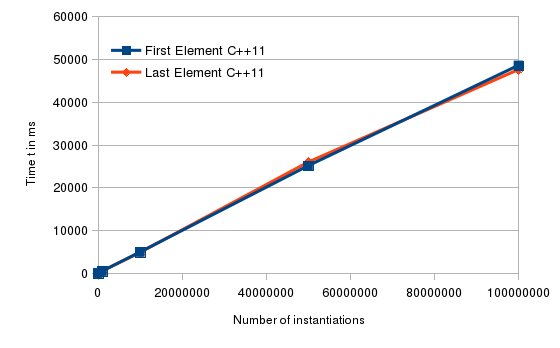
\includegraphics[width=\textwidth]{Images/LambdaFactoryTiming.png}}}
\caption{Lambda implementation timing}
\label{fig:lambdaImplementationTiming}
\end{figure}

\noindent With about 48 seconds for instantiating 100,000,000 objects (Figure \ref{fig:lambdaImplementationTiming}) the lambda implementation has a similar timing like C++11 implementation of the clone factory. Also the seek complexity is with T(n) = O(1) the same because of the use of an unordered map. The profiling output (Table \ref{tab:LambdaFactoryTimingDistributionCpp11}) of the lambda implementation shows that the use of smart pointers has with about 64\% and 30.7 seconds the biggest effect on the total execution time.

\begin{table}[h]\begin{center}
\begin{tabular}{|c|c|c|}\hline
\textbf{Category} & \textbf{Percentage} & \textbf{Time in s}\\
\hline
Factory & 24.80 & 11.78\\
\hline
Smart pointer & 64.71 & 30.73\\
\hline
Shape & 2.38 & 1.13\\
\hline
Main & 3.63 & 1.72\\
\hline
Other & 4.11 & 1.95\\
\hline
\end{tabular}
\caption{Lambda implementation timing distribution C++11}
\label{tab:LambdaFactoryTimingDistributionCpp11}
\end{center}\end{table}

\FloatBarrier

%----------------------------------------------------------------------------------------
%	Memory Consumption for Lambda implementation
%----------------------------------------------------------------------------------------
\subsection{Memory Consumption}\label{sec:memoryConsumptionLambdaFactory}

\begin{figure}[h]{}
\centering
\mbox{\frame{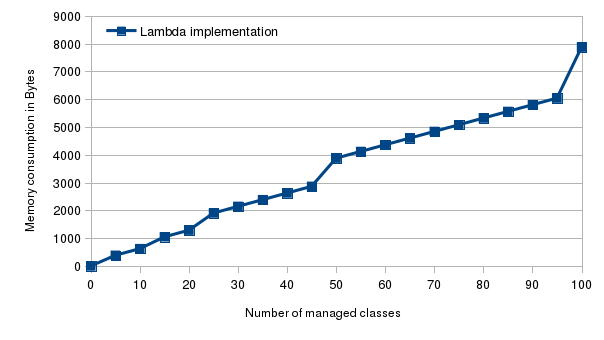
\includegraphics[width=\textwidth]{Images/FactoryPatternLambdaMemoryConsumption.png}}}
\caption{Lambda implementation memory consumption}
\label{fig:lambdaImplementationMemoryConsumption}
\end{figure}

\noindent On the first look, the lambda implementation of the factory shows exactly the same memory consumption (Figure \ref{fig:lambdaImplementationMemoryConsumption}) than the C++11 clone factory implementation (Figure \ref{fig:cloneFactoryMemoryConsumption}). But this is only true in case when the managed classes have minimum size. One advantage of the lambda implementation, compared with the clone factory implementation, is the managemend of classes instead of objects. This makes the memory consumption of the factory independent of the size of the managed classes. So, in case when the size of the classes rise, the memory consumption of the clone factory implementation also rises, but the lambda implementation stays constant.
\endgroup}
